
%!TEX root = handout.tex

% File names are changed quite often between tutorial so make them configurable at the top.
% Please escape whitespaces except before and after / as a path separator.
\newcommand{\WindowsKnimeInstallerName}{Windows / KNIME\ 4.1.1\ Installer\ (64bit).exe}	
\newcommand{\WindowsOpenMSInstallerName}{Windows / OpenMS-2.5.0-Win64.exe}	
\newcommand{\WindowsOpenMSPrereqInstallerName}{Windows / OpenMS-2.5-prerequisites-installer.exe}
\newcommand{\WindowsPrerequisitesLink}{https://abibuilder.informatik.uni-tuebingen.de/archive/openms/OpenMSInstaller/PrerequisitesInstaller/OpenMS-2.5-prerequisites-installer.exe}
\newcommand{\WindowsDefaultPWizFolder}{C: / Program\ Files / OpenMS-2.5.0 / share / OpenMS / THIRDPARTY / pwiz-bin}
\newcommand{\MacKnimeInstallerName}{Mac / knime\_4.1.0.app.macosx.cocoa.x86\_64.dmg}	
\newcommand{\MacOpenMSInstallerName}{Mac / OpenMS-2.5.0-macOS.dmg}
\newcommand{\KnimeUpdateSite}{http://update.knime.com/analytics-platform/4.1}
\newcommand{\KnimeTrustedSite}{http://update.knime.com/community-contributions/trusted/4.1}
\newcommand{\KnimeTrunkSite}{https://abibuilder.informatik.uni-tuebingen.de/archive/openms/knime-plugin/updateSite/nightly/}
\newcommand{\KnimeUSBUpdateSite}{file:/KNIMEUpdateSite/2.5.0/}

\setcounter{equation}{0}

%%%%%%%%%%%%%%%%%%%%%%%%%%%%%%%%%%%%%%%%%%%%%%%%%%%%%%%%%%%%%%%%%%%%%%%%%%%%%%%%
\section{Getting started}

\subsection{Installation}

Before we get started we will install OpenMS and KNIME. If you take part in a training session you will have likely received an USB stick from us that contains the required data and software. If we provide laptops with the software you may of course skip the installation process and continue reading the next section.

\subsubsection{Installation from the OpenMS USB stick}
Please choose the directory that matches your operating system and execute the installer. 

For example for \textbf{Windows} you call
\begin{itemize}
  \item the OpenMS installer: \directory{\WindowsOpenMSInstallerName}
  \item the KNIME installer:  \directory{\WindowsKnimeInstallerName}
  \item OpenMS prerequisites (Windows-only): After installation, before your first use of the OpenMS plugin in KNIME you will be asked to download it automatically if certain requirements are not found in your Windows registry. Alternatively, you can get a bundled version \href{\WindowsPrerequisitesLink}{here} or on the OpenMS USB stick (\directory{\WindowsOpenMSPrereqInstallerName}).
\end{itemize}

on \textbf{macOS} you call
\begin{itemize}
  \item the OpenMS installer: \directory{\MacOpenMSInstallerName}
  \item the KNIME installer: \directory{\MacKnimeInstallerName}
\end{itemize}

and follow the instructions. For the OpenMS installation on \textbf{macOS}, you need to accept the license drag and drop the OpenMS folder into your Applications folder.
\note{Due to increasing security measures for downloaded apps (e.g. path randomization) on \textbf{macOS} you might need to open TOPPView.app and TOPPAS.app while holding \keys{\ctrl} and accept the warning.
If the app still does not open, you might need to move them from \directory{Applications / OpenMS-2.5.0} to e.g. your Desktop and back.}
 On \textbf{Linux} you can extract KNIME to a folder of your choice and for TOPPView you need to install OpenMS via your package manager or build it on your own with the instructions under \href{https://www.openms.de/documentation}{www.openms.de/documentation}.
\note{If you have installed OpenMS on Linux or macOS via your package manager (for instance by installing the \texttt{OpenMS-2.5.0-Linux.deb} package), then you need to set the \texttt{OPENMS\_DATA\_PATH} variable to the directory containing the shared data (normally \texttt{/usr/share/OpenMS}). This must be done prior to running any TOPP tool.}

\subsubsection{Installation from the internet}
If you are working through this tutorial at home you can get the installers under the following links:
\begin{itemize}
  \item OpenMS: \href{https://www.openms.de/download/openms-binaries}{ https://www.openms.de/download/openms-binaries}
  \item KNIME: \href{https://www.knime.org/downloads/overview}{ https://www.knime.org/downloads/overview}
  \item OpenMS prerequisites (Windows-only): After installation, before your first use of the OpenMS plugin in KNIME you will be asked to download it automatically if certain requirements are not found in your Windows registry. Alternatively, you can get a bundled version \href{\WindowsPrerequisitesLink}{here}.
\end{itemize}
Choose the installers for the platform you are working on.

\subsection{Data conversion}
\label{Data_Conversion}

Each MS instrument vendor has one or more formats for storing the acquired data. Converting these data into an open format (preferably mzML) is the very first step when you want to work with open-source mass spectrometry software. A freely available conversion tool is \texttt{MSConvert}, which is part of a \texttt{ProteoWizard} installation. All files used in this tutorial \textbf{have already been converted to mzML} by us, so you do not need to perform the data conversion yourself.
However, we provide a small raw file so you can try the important step of raw data conversion for yourself.

\note{The OpenMS installation package for Windows automatically installs ProteoWizard, so you do not need to download and install it separately. Due to restrictions from the instrument vendors, file format conversion for most formats is \textbf{only possible on Windows} systems. In practice, performing the conversion to mzML on the acquisition PC connected to the instrument is usually the most convenient option.}

\noindent To convert raw data to mzML using \texttt{ProteoWizard} you can either use \texttt{MSConvertGUI} (a graphical user interface) or \texttt{msconvert} (a simple command line tool). Both tools are available in:
\newline
\directory{\WindowsDefaultPWizFolder}.
You can find a small RAW file on the USB stick:
\directory{Example\_Data / Introduction / datasets / raw}.

\subsubsection{MSConvertGUI}
\texttt{MSConvertGUI} (see Fig.~\ref{fig:MSConvertGUI}) exposes the main parameters for data conversion in a convenient graphical user interface.

\begin{figure}
\centering
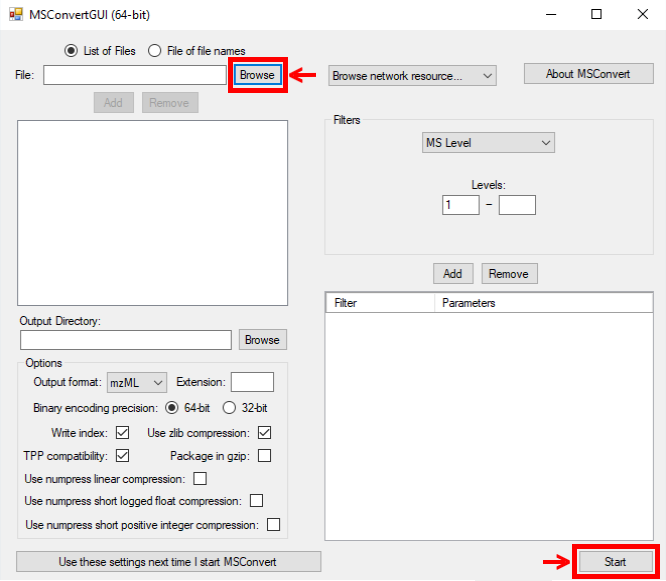
\includegraphics[width=12cm]{graphics/introduction/proteowizard.png}
\caption{\texttt{MSConvertGUI} (part of \texttt{ProteoWizard}), allows converting raw files to mzML. Select the raw files you want to convert by clicking on the browse button and then on \menu{Add}. Default parameters can usually be kept as-is. To reduce the initial data size, make sure that the peakPicking filter (converts profile data to centroided data (see Fig.~\ref{fig:ProfileCentroidData})) is listed, enabled (true) and applied to all MS levels (parameter "1-"). Start the conversion process by clicking on the \menu{Start} button.}
\label{fig:MSConvertGUI}
\end{figure}

\begin{figure}
\centering
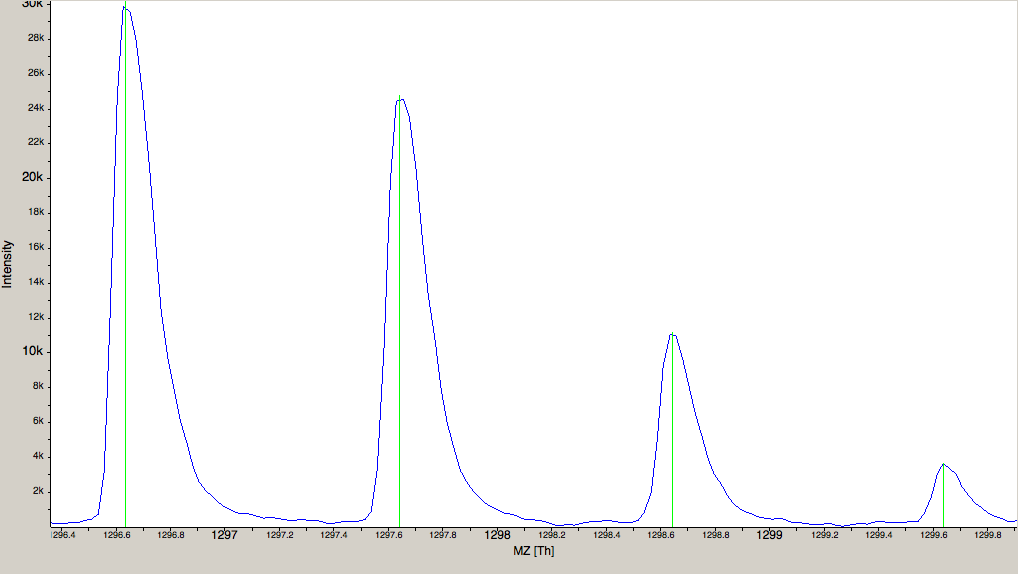
\includegraphics[width=12cm]{graphics/introduction/profilecentroided.png}
\caption{The amount of data in a spectra is reduced by peak picking. Here a profile spectrum (blue) is converted to centroided data (green). Most algorithms  from this point on will work with centroided data.}
\label{fig:ProfileCentroidData}
\end{figure}

\subsubsection{msconvert}
The \texttt{msconvert} command line tool has no user interface but offers more options than the application \texttt{MSConvertGUI}. Additionally, since it can be used within a batch script, it allows converting large numbers of files and can be much more easily automatized.

\noindent To convert and pick the file \textit{raw\_data\_file.RAW} you may write:

%% -{}- avoids latex ligatures
\noindent\menu{msconvert raw\_data\_file.RAW -{}-filter "peakPicking true 1-"}

\noindent in your command line.

\noindent To convert all RAW files in a folder may write:

\noindent\menu{msconvert *.RAW -o my\_output\_dir}

\note{To display all options you may type \menu{msconvert -{}-help}. Additional information is available on the ProteoWizard web page.}

\subsubsection{ThermoRawFileParser}

Recently the open-source platform independent ThermoRawFileParser tool has been developed. While Proteowizard and MSConvert are only available for Windows systems this new tool allows to also convert raw data on Mac or Linux.

\note{To learn more about the ThermoRawFileParser and how to use it in KNIME see Section \ref{sec:Minimal_Workflow}} 

%%%%%%%%%%%%%%%%%%%%%%%%%%%%%%%%%%%%%%%%%%%%%%%%%%%%%%%%%%%%%%%%%%%%%%%%%%%%%%%%

\subsection{Data visualization using \OPENMSTOOL{TOPPView}}
\label{Data_Visualization}

Visualizing the data is the first step in quality control, an essential tool in understanding the data, and of course an essential step in pipeline development.
OpenMS provides a convenient viewer for some of the data: \OPENMSTOOL{TOPPView}.

\begin{figure}
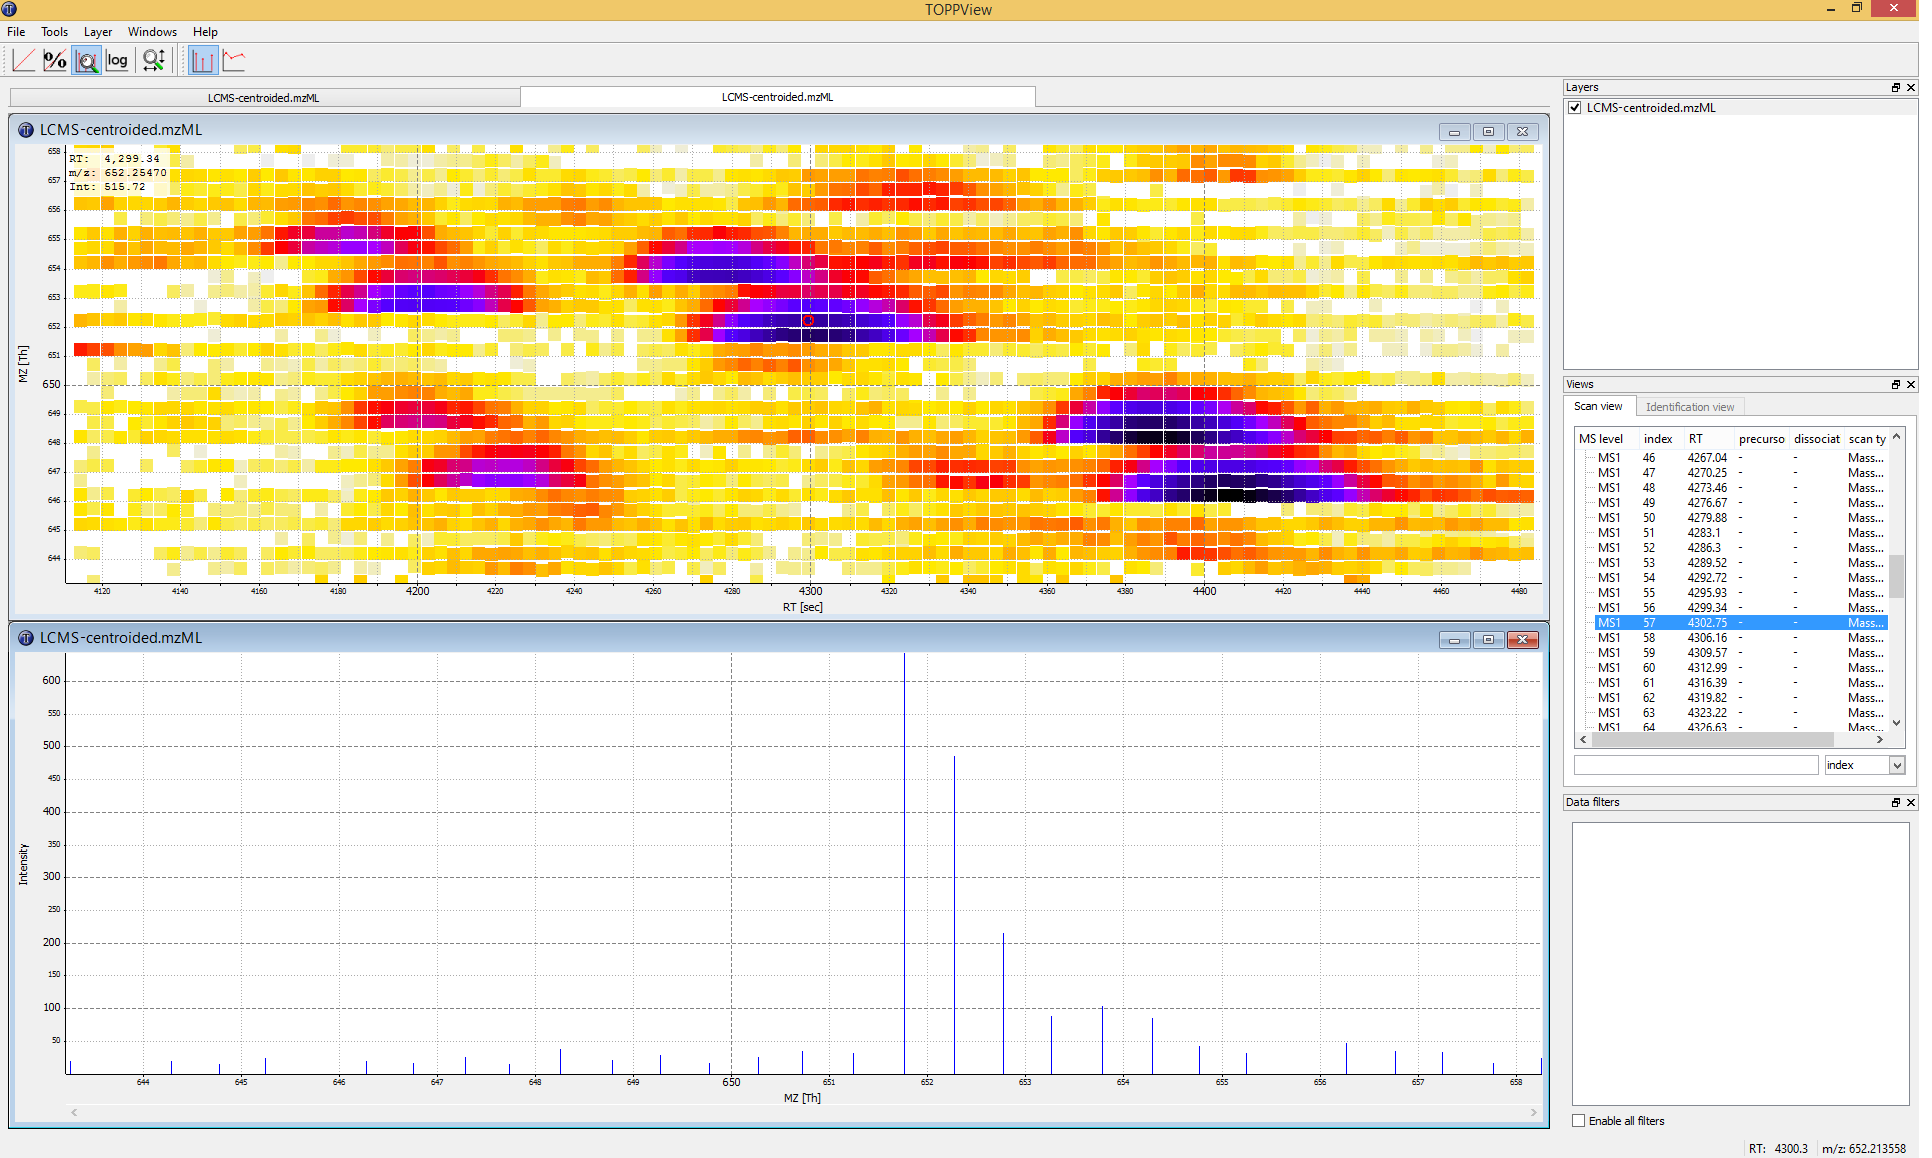
\includegraphics[width=\textwidth]{graphics/introduction/TOPPView.png}
\caption{TOPPView, the graphical application for viewing mass spectra and analysis results. Top window shows a small region of a peak map. In this 2D representation of the measured spectra, signals of eluting peptides are colored according to the raw peak intensities. The lower window displays an extracted spectrum (=scan) from the peak map. On the right side, the list of spectra can be browsed.}
\label{fig:toppview}
\end{figure}

\noindent We will guide you through some of the basic features of \OPENMSTOOL{TOPPView}. Please familiarize yourself with the key controls and visualization methods.
We will make use of these later throughout the tutorial. Let's start with a first look at one of the files of our tutorial data set. Note that conceptually, there are no differences in visualizing metabolomic or proteomic data. Here, we inspect a simple proteomic measurement:

\begin{figure}[!htb]
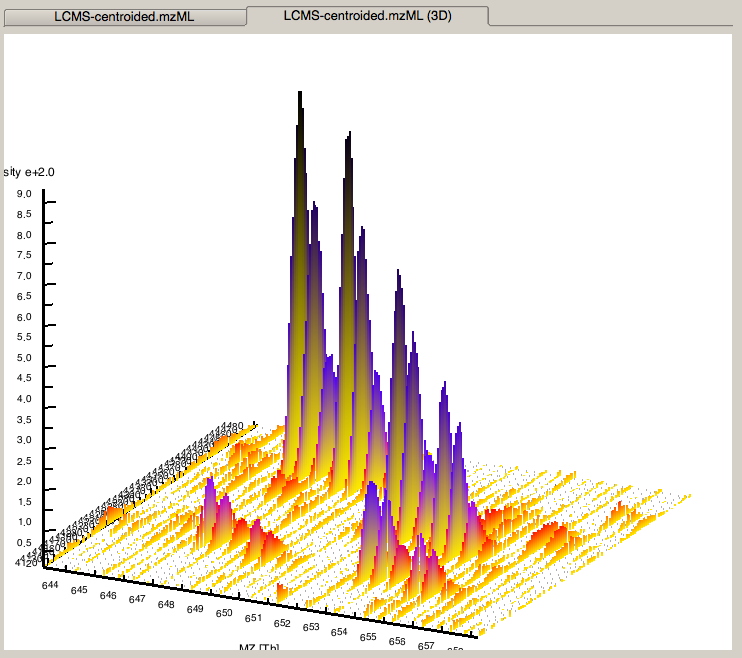
\includegraphics[width=0.75\textwidth]{graphics/introduction/3dview.png}
\caption{3D representation of the measured spectra, signals of eluting peptides are colored according to the raw peak intensities.}
\label{fig:toppview_3D}
\end{figure}


\begin{itemize}
\item Start \OPENMSTOOL{TOPPView} (see \textbf{Windows}' Start-Menu or \directory{Applications/OpenMS-2.4.0} on \textbf{macOS})
\item Go to \menu{File > Open File}, navigate to the directory where you copied the contents of the USB stick to,
      and select
      \directory{Example\_Data / Introduction / datasets / small / velos005614.mzML}
      . This file contains only a reduced LC-MS map \footnote{only a selected RT and m/z range
      was extracted using the TOPP tool \OPENMSTOOL{FileFilter}} of a label-free proteomic platelet measurement recorded on an Orbitrap velos.
      The other two mzML files contain technical replicates of this experiment.
      First, we want to obtain a global view on the whole LC-MS map - the default option \textit{Map view 2D} is the correct one and we can click the \menu{Ok} button. 
\item Play around.
\item Three basic modes allow you to interact with the displayed data: scrolling, zooming and measuring:
    \begin{itemize}
    \item Scroll mode
        \begin{itemize}
        \item Is activated by default (though each loaded spectra file is displayed zoomed out first, so you do not need to scroll).
        \item Allows you to browse your data by moving around in RT and m/z range.
        \item When zoomed in, you can scroll through the spectra. Click-drag on the current view.
        \item Arrow keys can be used to scroll the view as well.
        \end{itemize}
    \item Zoom mode
        \begin{itemize}
        \item Zooming into the data: either mark an area in the current view with your mouse while holding the left mouse
              button plus the \keys{\ctrlwin} key to zoom to this area
              or use your mouse wheel to zoom in and out.
        \item All previous zoom levels are stored in a zoom history. The zoom history can be traversed using
              \keys[,]{\ctrlwin,+} or \keys[,]{\ctrlwin,-} or the mouse wheel (scroll up and down).
        \item Pressing backspace \keys{\, \backspace \,\,} zooms out to show the full LC-MS map (and also resets the zoom history).
        \end{itemize}
    \item Measure mode
        \begin{itemize}
        \item It is activated using the \keys{\, \shift \,\,\, } (shift) key.
        \item Press the left mouse button down while a peak is selected and drag the mouse to
        			another peak to measure the distance between peaks.
        \item This mode is implemented in the 1D and 2D mode only.
        \end{itemize}
    \end{itemize}
\item Right click on your 2D map and select \menu{Switch to 3D view} and examine your
			data in 3D mode (see Fig. ~\ref{fig:toppview_3D})
			%TODO: Inconsitent buttons 2D 1D 3D
\item Go back to the 2D view. In 2D mode, visualize your data in different intensity normalization modes, use linear , percentage, snap and log-view (icons on the upper left tool bar). You can hover over the icons for additional information. 
\note{On \textit{macOS}, due to a bug in one of the external libraries used by OpenMS, you will see a small window of the 3D mode when switching to 2D. Close the 3D tab in order to get rid of it.}
\item In \OPENMSTOOL{TOPPView} you can also execute TOPP tools. Go to
			\menu{Tools > Apply tool (whole layer)} and choose a TOPP tool (e.g., \OPENMSTOOL{FileInfo}) and
			inspect the results.
\end{itemize}

\noindent Dependent on your data MS/MS spectra can be visualized as well (see Fig.\ref{fig:ms2}) . You can do so, by double-click on the MS/MS spectrum shown in scan view.
\newline
\begin{figure}[!htb]
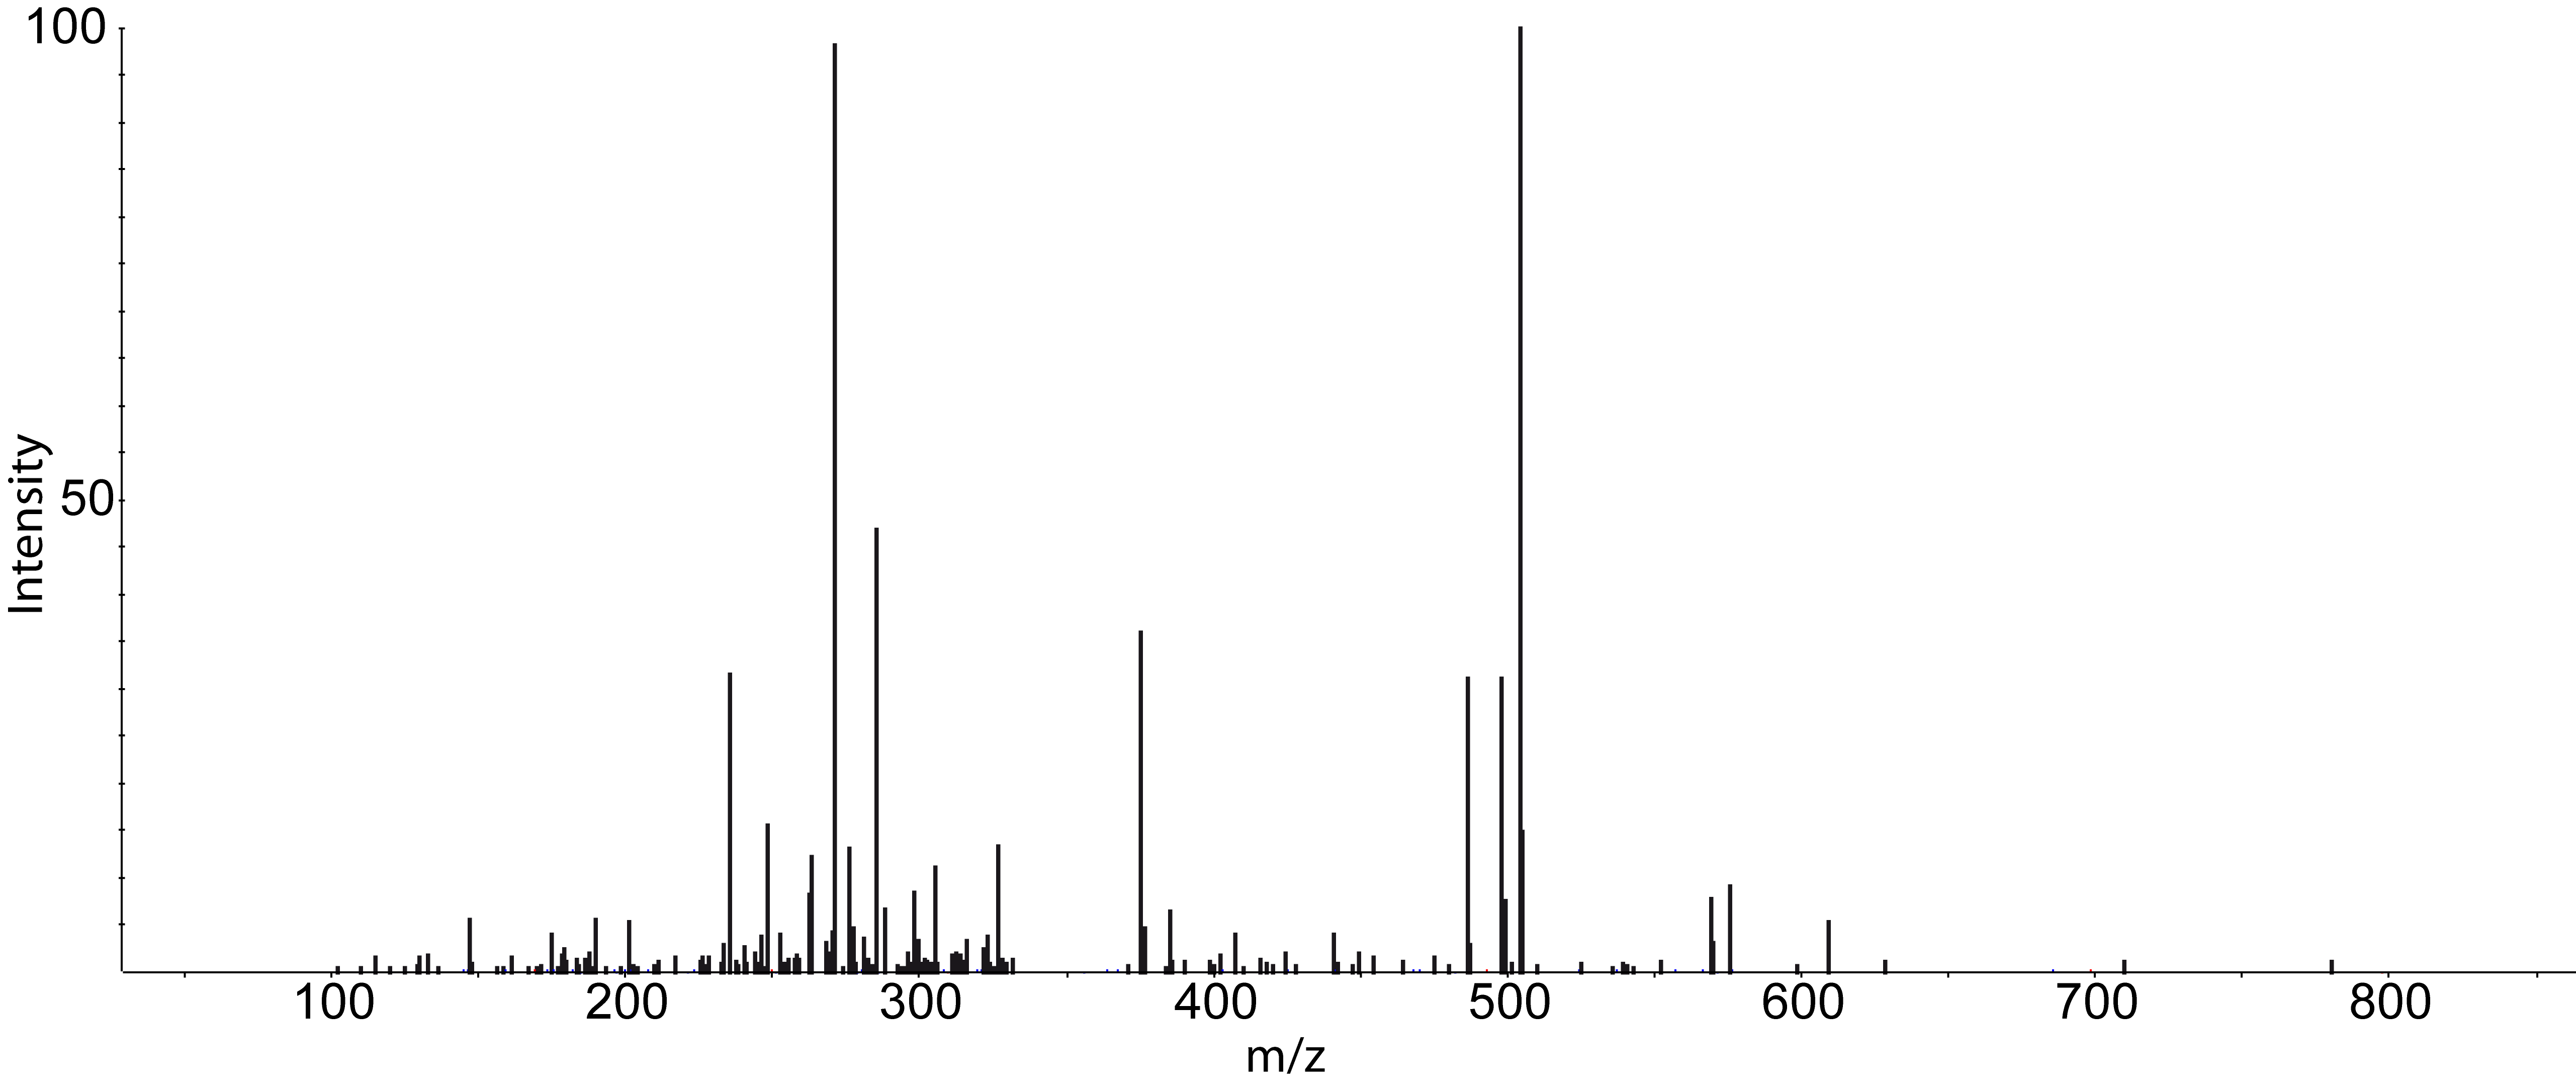
\includegraphics[width=0.75\textwidth]{graphics/introduction/ms2_introduction.png}
\caption{MS/MS spectrum}
\label{fig:ms2}
\end{figure}


%%%%%%%%%%%%%%%%%%%%%%%%%%%%%%%%%%%%%%%%%%%%%%%%%%%%%%%%%%%%%%%%%%%%%%%%%%%%%%%%

\subsection{Introduction to KNIME / OpenMS}
\label{KNIME_Intro}

Using OpenMS in combination with KNIME, you can create, edit, open, save, and run workflows
that combine TOPP tools with the powerful data analysis capabilities of KNIME. Workflows can
be created conveniently in a graphical user interface. The parameters of all involved
tools can be edited within the application and are also saved as part of the workflow.
Furthermore, KNIME interactively performs validity checks during the workflow editing
process, in order to make it more difficult to create an invalid workflow.
\newline
\noindent Throughout most parts of this tutorial you will use KNIME to create and
execute workflows. The first step is to make yourself familiar with KNIME. Additional
information on basic usage of KNIME can be found on the KNIME
\href{https://tech.knime.org/knime}{Getting Started page}. However,
the most important concepts will also be reviewed in this tutorial.

\subsubsection{Plugin and dependency installation}
\label{Install_plugins}
Before we can start with the tutorial we need to install all the required extensions for KNIME. Since KNIME 3.2.1 the program automatically
detects missing plugins when you open a workflow but to make sure that the right source for the OpenMS plugin is chosen, please follow the instructions here.
First, we install some additional extensions that are required by our OpenMS nodes or used in the Tutorials e.g. for visualization and file handling.
\begin{enumerate}
\item Click on \menu{Help > Install New Software...}
\item From the \menu{Work with:} drop-down list select \menu{\KnimeUpdateSite}
\item Now select the following plugins from the \textit{KNIME \& Extensions} category
    \begin{itemize}
    \item KNIME Base Chemistry Types \& Nodes
    \item KNIME Chemistry Add-Ons
    \item KNIME File Handling Nodes (required for OpenMS nodes in general)
    \item KNIME Interactive R Statistics Integration
    \item KNIME Report Designer
    \item KNIME SVG Support
%    \item KNIME XLS Support not needed anymore (integrated in e.g. KNIME 3.2.1)
%    \item KNIME XML-Processing (integrated in e.g. KNIME 3.2.1)
%    \item KNIME Math Expression (JEP) (integrated in e.g. KNIME 3.2.1)
    \end{itemize}
%\item And the following plugin from the \textit{Marvin Chemistry Extensions (donated by Infocom \& Chemaxon)} category
%    \begin{itemize}
%    \item ChemAxon/Infocom Marvin Extensions Feature
%    \end{itemize}
\item Click on \menu{Next} and follow the instructions (you may but don't need to restart KNIME now)
\item Click again on \menu{Help > Install New Software...}
\item From the \menu{Work with:} drop-down list select \\\menu{\KnimeTrustedSite}
\item Now select the following plugin from the "KNIME Community Contributions - Cheminformatics" category 	
    \begin{itemize}
    \item     RDKit KNIME integration
    \end{itemize}	
\item Click on \menu{Next} and follow the instructions and after a restart of KNIME the dependencies will be installed.
\end{enumerate}

%Now you need to decide which OpenMS nodes you want to install. You may choose between the stable, well-tested release or the unstable, nightly release with extended functionality.

\noindent In addition, we need to install R for the statistical downstream analysis. Choose the directory that matches your operating system, double-click the R installer and follow the instructions. We recommend to use the default settings whenever possible. On macOS you also need to install XQuartz from the same directory.\\

\noindent Afterwards open your R installation. If you use Windows, you will find an "R x64 3.6.X" icon on your desktop. If you use macOS, you will find R in your Applications folder. In R type the following lines (you might also copy them from the file \directory{R / install\_R\_packages.R} folder on the USB stick):
\begin{lstlisting}[aboveskip=8pt]
  install.packages('Rserve',,"http://rforge.net/",type="source")
  install.packages("Cairo")
  install.packages("devtools")
  install.packages("ggplot2")
  install.packages("ggfortify")
  if (!requireNamespace("BiocManager", quietly = TRUE))
	install.packages("BiocManager")
  BiocManager::install()
  BiocManager::install(c("MSstats"))
\end{lstlisting}

\noindent In KNIME, click on \menu{KNIME > Preferences}, select the category \menu{KNIME > R} and set the "Path to R Home" to your installation path. You can use the following settings, if you installed R as described above:
\begin{itemize}
\item Windows: C: \textbackslash Program Files \textbackslash R \textbackslash R-3.6.X (where X is the version you used to install the above libraries)
\item macOS: /Library/Frameworks/R.framework/Versions/3.6/Resources 
\end{itemize}

\noindent You are now ready to install the OpenMS nodes.

\begin{itemize}
	\item Open KNIME.
	\item Click on \menu{Help > Install New Software...}
\end{itemize}
%\iftoggle{isprerelease}
%{
%\note{For this tutorial we use the \textbf{bleeding edge, nightly release} version of OpenMS because it corresponds to a prerelease of the new OpenMS version. While not being a full release, it was nevertheless intensively tested to ensure its functionality for this tutorial. For regular use we still recommend using the latest stable OpenMS release. Please also note that some of the workflows shown here require new functionality contained only in the prerelease version of OpenMS. These will likely not work if transferred to the current stable, but older OpenMS version.}
%
%Instructions for the bleeding edge, nightly release:
%\begin{itemize}
% % If you base the tutorial on the nightly contributions (not recommended - more of a emergency measure)
%  \item \label{it:add_site} In the now open dialog choose \menu{Add...} (in the upper right corner of the dialog) to define a new update site. In the opening dialog enter the following details. \\
%  \textit{Name:} \texttt{Trunk Community Contributions} \\
%  \textit{Location:} \menu{\KnimeTrunkSite}
%  \item \label{it:select_site} After pressing \keys{OK} KNIME will show you all the contents of the added Update Site.
%  \item \textbf{Note:} From now on, you can use this repository for plugins in the \menu{Work with:} drop-down list.
%  \item Select the \textbf{OpenMS} nodes in the category: \\ "KNIME Community Contributions - Bioinformatics \& NGS" and click \keys{Next}.
%  \item Follow the instructions and after a restart of KNIME the OpenMS nodes will be available in the Node repository under “Community Nodes”.
%\end{itemize}
%}
%{
%Instructions for the stable release (recommended):
%\begin{itemize}
%  \item From the \menu{Work with:} drop-down list select the \\ \menu{\KnimeTrustedSite}
%  \item Select the \textbf{OpenMS} nodes in the category: \\ "KNIME Community Contributions - Bioinformatics \& NGS" and click \keys{Next}.
%  \item Follow the instructions and after a restart of KNIME the OpenMS nodes will be available in the Node repository under “Community Nodes”.
%\end{itemize}

We included a custom KNIME update site to install the OpenMS KNIME plugins from the USB stick. If you do not have a stick available, please see below.

\begin{itemize}
 % If you base the tutorial on the nightly contributions (not recommended - more of a emergency measure)
  \item \label{it:add_site} In the now open dialog choose \menu{Add...} (in the upper right corner of the dialog) to define a new update site. In the opening dialog enter the following details. \\
  \textit{Name:} \texttt{OpenMS 2.4 UpdateSite} \\
  \textit{Location:}  \KnimeUSBUpdateSite \\
  \item \label{it:select_site} After pressing \keys{OK} KNIME will show you all the contents of the added Update Site.
  \item \textbf{Note:} From now on, you can use this repository for plugins in the \menu{Work with:} drop-down list.
  \item Select the \textbf{OpenMS} nodes in the "Uncategorized" category and click \keys{Next}.
  \item Follow the instructions and after a restart of KNIME the OpenMS nodes will be available in the Node repository under “Community Nodes”.
\end{itemize}

Alternatively, you can try these steps that will install the OpenMS KNIME plugins from the internet. Note that download can be slow.

\begin{itemize}
 % If you base the tutorial on the nightly contributions (not recommended - more of a emergency measure)
  \item \label{it:add_site} In the now open dialog choose \menu{Add...} (in the upper right corner of the dialog) to define a new update site. In the opening dialog enter the following details. \\
  \textit{Name:} \texttt{OpenMS 2.5 UpdateSite} \\
  \textit{Location:} 
\end{itemize}  
  \menu{\KnimeTrunkSite}
\begin{itemize}
  \item \label{it:select_site} After pressing \keys{OK} KNIME will show you all the contents of the added Update Site.
  \item \textbf{Note:} From now on, you can use this repository for plugins in the \menu{Work with:} drop-down list.
  \item Select the \textbf{OpenMS} nodes in the "Uncategorized" category and click \keys{Next}.
  \item Follow the instructions and after a restart of KNIME the OpenMS nodes will be available in the Node repository under “Community Nodes”.
\end{itemize}
%}

\subsubsection{KNIME concepts}
\label{KNIME_concepts}

A \textbf{workflow} is a sequence of computational steps applied to a single or multiple input data to process and analyze the data.
In KNIME such workflows are implemented graphically by connecting so-called \textbf{nodes}.
A node represents a single analysis step in a workflow.
Nodes have input and output \textbf{ports} where the data enters the node or the results are provided for other nodes after processing, respectively.
KNIME distinguishes between different port types, representing different types of data.
The most common representation of data in KNIME are tables (similar to an excel sheet).
Ports that accept tables are marked with a small triangle.
For OpenMS nodes, we use a different port type, so called \textbf{file ports}, representing complete files.
Those ports are marked by a small blue box.
Filled blue boxes represent mandatory inputs and empty blue boxes optional inputs. The same holds for output ports, despite you can deactivate them
in the configuration dialog (double-click on node) under the OutputTypes tab. After execution, deactivated ports will be marked with a red cross and downstream nodes
will be inactive (not configurable).\\
A typical OpenMS workflow in KNIME can be divided in two conceptually different parts:
\begin{itemize}
\item
Nodes for signal and data processing, filtering and data reduction. Here, files are passed between nodes. Execution times of the individual steps are typically longer for these types of nodes as they perform the main computations. 
\item
Downstream statistical analysis and visualization. Here, tables are passed between nodes and mostly internal KNIME nodes or nodes from third-party statistics plugins are used. The transfer from files (produced by OpenMS) and tables usually happens with our provided Exporter and Reader nodes (e.g. MzTabExporter followed by MzTabReader).
\end{itemize}
Moreover, nodes can have three different states, indicated by the small traffic light below the node.

\begin{itemize}
\item
Inactive, failed, and not yet fully configured nodes are marked red.
\item
Configured but not yet executed nodes are marked yellow.
\item
Successfully executed nodes are marked green.
\end{itemize}

If the node execution fails, the node will switch to the red state. Other anomalies and warnings like missing information or empty results 
will be presented with a yellow exclamation mark above the traffic light.
Most nodes will be configured as soon as all input ports are connected. Some nodes need to know about the output of the predecessor and may stay red until the predecessor was executed.
If nodes still remain in a red state, probably additional parameters have to be provided in the configuration dialog that can neither be guessed from the data nor filled with sensible defaults.
In this case, or if you want to customize the default configuration in general, you can open the configuration dialog of a node with a double-click on the node.
For all OpenMS nodes you will see a configuration dialog like the one shown in \cref{fig:knime_configure}.
\note{OpenMS distinguishes between normal parameters and advanced parameters.
Advanced parameters are by default hidden from the users since they should only rarely be customized.
In case you want to have a look at the parameters or need to customize them in one of the tutorials you can show them by clicking on the checkbox \menu{Show advanced parameter} in the lower part of the dialog. Afterwards the parameters are shown in a light gray color.} 
The dialog shows the individual parameters, their current value and type, and, in the lower part of the dialog, the 
documentation for the currently selected parameter. Please also note the tabs on the top of the configuration dialog. 
In the case of OpenMS nodes, there will be another tab called \textit{OutputTypes}. It contains dropdown menus for 
every output port that let you select the output filetype that you want the node to return (if the tool supports 
it). For optional output ports you can select \textit{Inactive} such that the port is crossed out after execution and 
the associated generation of the file and possible additional computations are not performed. Note that this will 
deactivate potential downstream nodes connected to this port.

\begin{figure}
\centering
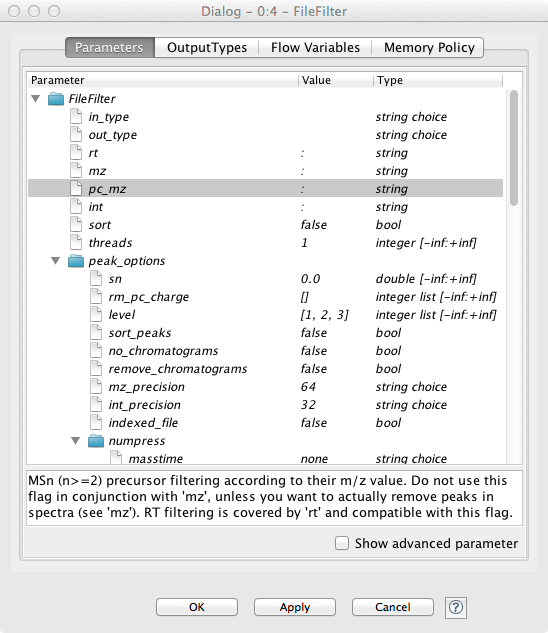
\includegraphics[width=0.5\textwidth]{graphics/knime_setup/knime_configure_dialog}
\caption{Node configuration dialog of an OpenMS node.}
\label{fig:knime_configure}
\end{figure}

\subsubsection{Overview of the graphical user interface}

\begin{figure}
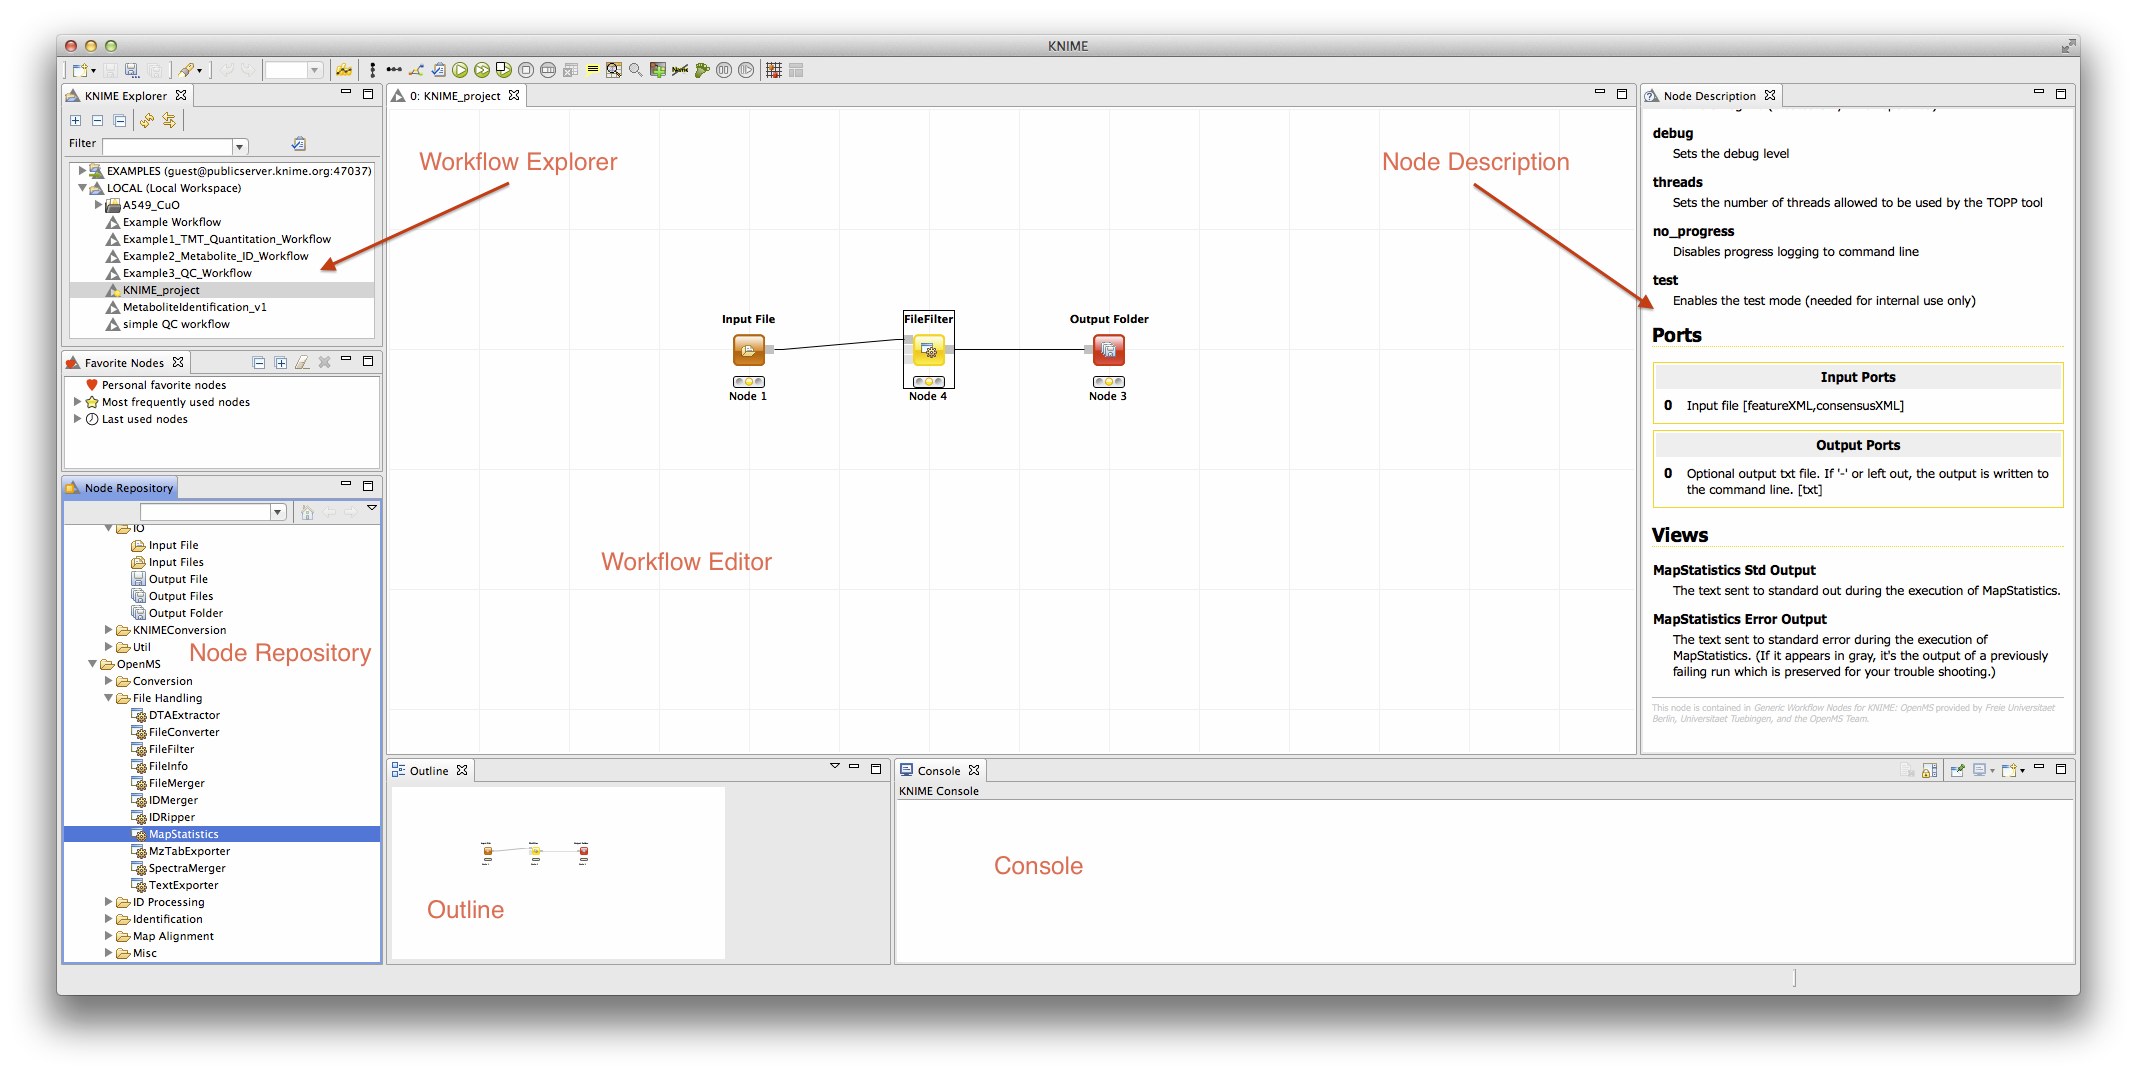
\includegraphics[width=\textwidth]{graphics/knime_setup/knime_workbench_marked}
\caption{The KNIME workbench.}
\label{fig:knime_workbench}
\end{figure}

The graphical user interface (GUI) of KNIME consists of different components or so-called panels that are shown in \cref{fig:knime_workbench}.
We will briefly introduce the individual panels and their purposes below.

\begin{description}
\item[Workflow Editor:]
The workflow editor is the central part of the KNIME GUI.
Here you assemble the workflow by adding nodes from the Node Repository via "drag \& drop". For quick creation of a 
workflow, note that double-clicking on 
a node in the repository automatically connects it to the selected node in the workbench (connecting all the inputs 
with as many fitting outputs of the last node).
Manually, nodes can be connected by clicking on the output port of one node and dragging the edge until releasing the 
mouse at the desired input port of the next node. Deletions are possible by selecting nodes and/or edges and pressing 
\keys{Del} or (\keys{Fn}+)\keys{Backspace} depending on your OS and settings. Multiselection happens via dragging 
rectangles with the mouse or adding elements to the selection by clicking them while holding down \keys{Ctrl}.

\item[KNIME Explorer:]
Shows a list of available workflows (also called workflow projects).
You can open a workflow by double-clicking it.
A new workflow can be created with a right-click in the Workflow Explorer followed by choosing \menu{New KNIME 
Workflow...} from the appearing context menu.
Remember to save your workflow often with the \menu{Ctrl}+\menu{S} shortcut.

\item[Workflow Coach (since KNIME 3.2.1):]
Shows a list of suggested following nodes, based on the last added/clicked nodes.
When you are not sure which node to choose next, you have a reasonable suggestion based on other users behavior 
there. Connect them to the last node with a double-click.

\item[Node Repository:]
Shows all nodes that are available in your KNIME installation.
Every plugin you install will provide new nodes that can be found here.
The OpenMS nodes can be found in \menu{Community Nodes > OpenMS}.
Nodes for managing files (e.g., Input Files or Output Folders) can be found in \menu{Community Nodes > GenericKnimeNodes}.
You can search the node repository by typing the node name into the small text box in the upper part of the node repository.

\item[Outline:]
The Outline panel contains a small overview of the complete workflow. While of limited use when working on a small 
workflow, this feature is very helpful as soon as the workflows get bigger. You can adjust the zoom level of the 
explorer by adjusting the percentage in the toolbar at the top of KNIME.

\item[Console:]
In the console panel warning and error messages are shown.
This panel will provide helpful information if one of the nodes failed or shows a warning sign.

\item[Node Description:]
As soon as a node is selected, the Node Description window will show the documentation of the node including 
documentation for all its parameters and especially their in- and outputs, such that you know what types of data 
nodes may produce or expect.
For OpenMS nodes you will also find a link to the tool page of the online documentation.

\end{description}

\subsubsection{Creating workflows}
\label{sec:create_workflows}

Workflows can easily be created by a right click in the Workflow Explorer followed by clicking on \menu{New KNIME Workflow...}.

\subsubsection{Sharing workflows}
\label{sec:sharing_workflows}

To be able to share a workflow with others, KNIME supports the import and export of complete workflows.
To export a workflow, select it in the Workflow Explorer and select \menu{File > Export KNIME Workflow...}.
KNIME will export workflows as a \textit{knwf} file containing all the information on nodes, their connections, and their parameter configuration.
Those \textit{knwf} files can again be imported by selecting \menu{File > Import KNIME Workflow...}.

\note{For your convenience we added all workflows discussed in this tutorial to the \directory{Workflows} folder on the USB Stick. Additionally, the
workflow files can be found on our \href{https://github.com/OpenMS/Tutorials}{GitHub repository}.
If you want to check your own workflow by comparing it to the solution or got stuck, simply import the full workflow from the corresponding \textit{knwf} file and after that double-click it in your KNIME Workflow repository to open it.}

\subsubsection{Duplicating workflows}
\label{sec:duplicate-wf}

In this tutorial, a lot of the workflows will be created based on the workflow from a previous task.
To keep the intermediate workflows, we suggest you create copies of your workflows so you can see the progress.
To create a copy of your workflow, save it, close it and follow the next steps.

\begin{itemize}
\item
Right click on the workflow you want to create a copy of in the Workflow Explorer and select \menu{Copy}.
\item
Right click again somewhere on the workflow explorer and select \menu{Paste}.
\item
This will create a workflow with same name as the one you copied with a (2) appended.
\item
To distinguish them later on you can easily rename the workflows in the Workflow Explorer by right clicking on the workflow and selecting \menu{Rename}. \note{To rename a workflow it has to be closed, too.}
\end{itemize}

\subsubsection{A minimal workflow}
\label{sec:Minimal_Workflow}

Let us now start with the creation of our very first, very simple workflow.
As a first step, we will gather some basic information about the data set before starting the
actual development of a data analysis workflow. This minimal workflow can also be used to check if all requirements 
are met and that your system is compatible.

\begin{itemize}
\item
Create a new workflow.
\item Add an \KNIMENODE{Input File} node and an \KNIMENODE{Output Folder} node (to be found in \menu{Community Nodes > GenericKnimeNodes > IO} and a \KNIMENODE{FileInfo} node (to be found in the category \menu{Community Nodes > OpenMS > File Handling}) to the workflow.
\item Connect the \KNIMENODE{Input File} node to the \KNIMENODE{FileInfo} node, and the first output port of the \KNIMENODE{FileInfo} node to the \KNIMENODE{Output Folder} node.
\note{In case you are unsure about which node port to use, hovering the cursor over the port in question will display the port name and what kind of input it expects.}
The complete workflow is shown in \cref{fig:knime_minimal}.
FileInfo can produce two different kinds of output files.
\item All nodes are still marked red, since we are missing an actual input file.
Double-click the Input File node and select \menu{Browse}.
In the file system browser select \directory{Example\_Data / Introduction / datasets / tiny / velos005614.mzML} and click \menu{Open}.
Afterwards close the dialog by clicking \menu{Ok}.
\note{Make sure to use the ``tiny'' version this time, not ``small'', for the sake of faster workflow execution.}
\item The \KNIMENODE{Input File} node and the \KNIMENODE{FileInfo} node should now have switched to yellow, but the \KNIMENODE{Output Folder} node is still red.
Double-click on the \KNIMENODE{Output Folder} node and click on \menu{Browse} to select an output directory for the generated data.
\item Great! Your first workflow is now ready to be run. Press \keys{\shift + F7} (shift key + F7; or the button with multiple green triangles in the KNIME Toolbar) to execute the complete workflow.
You can also right click on any node of your workflow and select \menu{Execute} from the context menu.
\item The traffic lights tell you about the current status of all nodes in your workflow.
Currently running tools show either a progress in percent or a moving blue bar, nodes waiting for data show the small word ``queued'', and successfully executed ones become green.
If something goes wrong (e.g., a tool crashes), the light will become red.
\item In order to inspect the results, you can just right-click the \KNIMENODE{Output Folder} node and select \menu{View: Open the output folder}.
You can then open the text file and inspect its contents.
You will find some basic information of the data contained in the mzML file, e.g., the total number of spectra and peaks, the RT and m/z range, and how many MS1 and MS2 spectra the file contains.
\end{itemize}

\begin{figure}
\centering
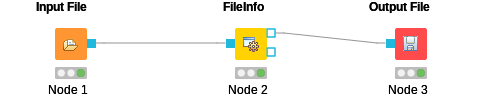
\includegraphics[width=0.59\textwidth]{graphics/knime_setup/Minimal_FileInfo}
\caption{A minimal workflow calling FileInfo on a single file.}
\label{fig:knime_minimal}
\end{figure}


Workflows are typically constructed to process a large number of files automatically.
As a simple example, consider you would like to convert multiple Thermo Raw files into the mzML format.
We will now modify the workflow to compute the same information on three different files and then write the output files to a folder.

\begin{itemize}
\item
We start from the previous workflow.
\item
First we need to replace our single input file with multiple files.
Therefore we add the \KNIMENODE{Input Files} node from the category \menu{Community Nodes > GenericKnimeNodes > IO}.
\item
To select the files we double-click on the \KNIMENODE{Input Files} node and click on \menu{Add}.
In the filesystem browser we select all three files from the directory \directory{Example\_Data / Introduction / datasets / tiny / }.
And close the dialog with \menu{Ok}.
\item
We now add two more nodes: the \KNIMENODE{ZipLoopStart} and the \KNIMENODE{ZipLoopEnd} node from the category \menu{Community Nodes > GenericKnimeNodes > Flow}. 
\item
Afterwards we connect the \KNIMENODE{Input Files} node to the first port of the \KNIMENODE{ZipLoopStart} node, the first port of the \KNIMENODE{ZipLoopStart} node to the \KNIMENODE{FileConverter} node, the first output port of the \KNIMENODE{FileConverter} node to the first input port of the \KNIMENODE{ZipLoopEnd} node, and the first output port of the \KNIMENODE{ZipLoopEnd} node to the \KNIMENODE{Output Folder} node (NOT to the \KNIMENODE{Output File}).
The complete workflow is shown in \cref{fig:knime_minimal_loop}
\item
The workflow is already complete.
Simply execute the workflow and inspect the output as before.
\end{itemize}

In case you had trouble to understand what ZipLoopStart and ZipLoopEnd do - here is a brief explanation:
\begin{itemize}
\item
The  \KNIMENODE{Input Files} node passes a list of files to the \KNIMENODE{ZipLoopStart} node.
\item
The \KNIMENODE{ZipLoopStart} node takes the files as input, but passes the single files sequentially (that is: one after the other) to the next node. 
\item
The \KNIMENODE{ZipLoopEnd} collects the single files that arrive at its input port. After all files have been processed, the collected files are passed again as file list to the next node that follows.
\end{itemize}

\begin{figure}
\centering
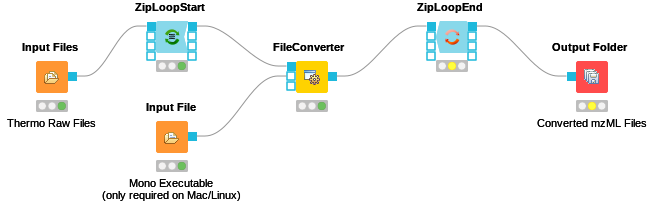
\includegraphics[width=\textwidth]{graphics/knime_setup/Minimal_RawFileConverter_Loop}
\caption{A minimal workflow calling the FileConverter on multiple Thermo Raw files in a loop.}
\label{fig:knime_minimal_loop}
\end{figure}

\subsubsection{Digression: Working with chemical structures}
Metabolomics analyses often involve working with chemical structures. Popular cheminformatic toolkits such as RDKit~\cite{rdkit} or CDK~\cite{cdk} are available as KNIME plugins and allow us to work with chemical structures directly from within KNIME. In particular, we will use KNIME and RDKit to visualize a list of compounds and filter them by predefined substructures. Chemical structures are often represented as SMILES (\textbf{S}implified \textbf{m}olecular \textbf{i}nput \textbf{l}ine \textbf{e}ntry \textbf{s}pecification), a simple and compact way to describe complex chemical structures as text. For example, the chemical structure of L-alanine can be written as the SMILES string C[C@H](N)C(O)=O. As we will discuss later, all OpenMS tools that perform metabolite identification will report SMILES as part of their result, which can then be further processed and visualized using RDKit and KNIME.

\begin{figure}
\centering
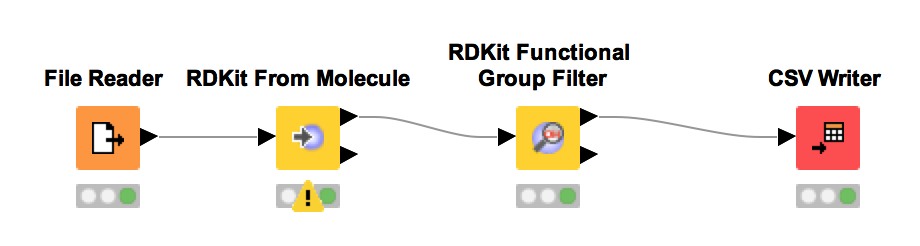
\includegraphics[width=\textwidth]{graphics/metabo/structures_filter_workflow.png}
\caption{Workflow to visualize a list of SMILES strings and filter them by predefined substructures.}
\label{fig:structures_filter_workflow}
\end{figure}

\noindent Perform the following steps to build the workflow shown in in Fig.~\ref{fig:structures_filter_workflow}. You will use this workflow to visualize a list of SMILES strings and filter them by predefined substructures:

\begin{itemize}
\item Add the node \KNIMENODE{File Reader}, open the node configuration dialog and select the file \directory{smiles.csv}. This file has been exported from the Human Metabolome Database (HMDB) and contains the portion of the human metabolome that has been detected and quantified. The file preview on the bottom of the dialog shows that each compound is given by its HMDB accession, compound name, and SMILES string. Click on the column header 'SMILES' to change its properties. Change the column type from 'string' to 'smiles' and close the dialog with \menu{Ok}. Afterwards the SMILES column will be visualized as chemical structures instead of text directly within all KNIME tables.

\item Add the node \KNIMENODE{RDKit From Molecule} and connect it to the  \KNIMENODE{File Reader}. This node will use the provided SMILES strings to add an additional column that is required by RDKit.

\item Add the node \KNIMENODE{RDKit Functional Group Filter} and open the node configuration dialog. You can use this dialog to filter the compounds by any combination of functional groups. In this case we want to find all compounds that contain at least one aromatic carboxylic acid group. To do this, set this group as active and choose '>=' and '1'.

\item Connect the first output port (Molecules passing the filter) to a \KNIMENODE{CSV Writer} node to save the filtered metabolites to a file. Right click \KNIMENODE{RDKit Functional Group Filter} and select the view 'Molecules passing the filter' to inspect the selected compounds in KNIME. How many compounds pass the chosen filter (see Fig.~\ref{fig:structures_filter_results})?

\begin{figure}
\centering
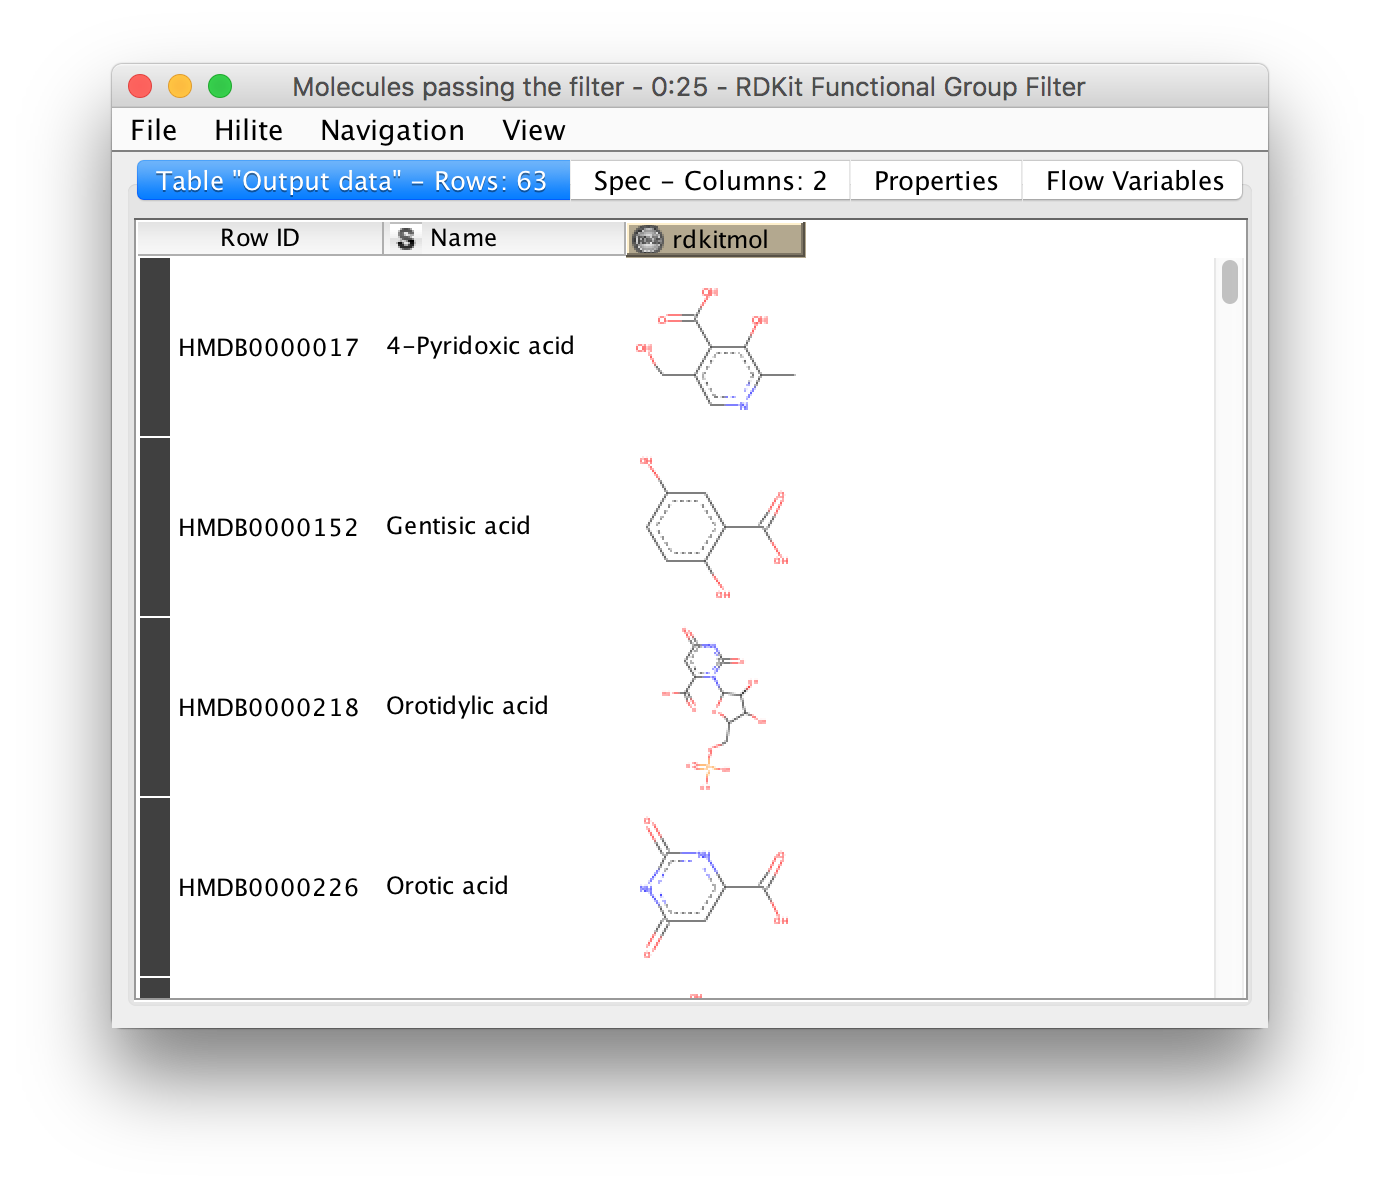
\includegraphics[width=0.59\textwidth]{graphics/metabo/structures_filter_results.png}
\caption{Resulting list of compounds that contains at least one aromatic carboxylic acid group.}
\label{fig:structures_filter_results}
\end{figure}

\end{itemize}


\subsubsection{Advanced topic: Metanodes}

Workflows can get rather complex and may contain dozens or even hundreds of nodes. KNIME provides a simple way to improve handling and clarity of large workflows:

\KNIMENODE{Metanodes} allow to bundle several nodes into a single \KNIMENODE{Metanode}.

\begin{task}
Select multiple nodes (e.g. all nodes of the ZipLoop including the start and end node). To select a set of nodes, draw a rectangle around them with the left mouse button or hold \keys{Ctrl} to add/remove single nodes from the selection. \textbf{Pro-tip:} There is a \menu{Select Loop} option when you right-click a node in a loop, that does exactly that for you. Then, open the context menu (right-click on a node in the selection) and select \menu{Create Metanode}. Enter a caption for the \KNIMENODE{Metanode}. The previously selected nodes are now contained in the \KNIMENODE{Metanode}. Double-clicking on the \KNIMENODE{Metanode} will display the contained nodes in a new tab window. 
\end{task}

%TODO: Check what is going on here with Metanode options! Wrap, ceate, freeze
%TODO: Check component 
\begin{task}
Create the Metanode to let it behave like an encapsulated single node. First select the \KNIMENODE{Metanode}, 
open the context menu (right-click) and select \menu{Metanode > Wrap}. The differences between Metanodes and their 
wrapped counterparts are marginal (and only apply when exposing user inputs and workflow variables). Therefore we 
suggest to use standard Metanodes to clean up your workflow and cluster common subparts until you actually notice 
their limits.
\end{task}

\begin{task}
Undo the packaging. First select the \KNIMENODE{(Wrapped) Metanode}, open the context menu (right-click) and select \menu{(Wrapped) Metanode > Expand}.
\end{task}

\subsubsection{Advanced topic: R integration}

KNIME provides a large number of nodes for a wide range of statistical analysis, machine learning, data processing, 
and visualization. Still, more recent statistical analysis methods, specialized visualizations or cutting edge 
algorithms may not be covered in KNIME. In order to expand its capabilities beyond the readily available nodes, 
external scripting languages can be integrated. In this tutorial, we primarily use scripts of the powerful 
statistical computing language R. Note that this part is considered advanced and might be difficult to follow if you 
are not familiar with R. In this case you might skip this part.

\KNIMENODE{R View (Table)} allows to seamlessly include R scripts into KNIME. We will demonstrate on a minimal 
example how such a script is integrated.

\begin{task}
First we need some example data in KNIME, which we will generate using the \KNIMENODE{Data Generator} node. You can 
keep the default settings and execute the node. The table contains four columns, each containing random coordinates 
and one column containing a cluster number (Cluster\_0 to Cluster\_3). Now place a \KNIMENODE{R View (Table)} node 
into the workflow and connect the upper output port of the \KNIMENODE{Data Generator} node to the input of the 
\KNIMENODE{R View (Table)} node. Right-click and configure the node.
If you get an error message like "Execute failed: R\_HOME does not contain a folder with name 'bin'." or "Execution 
failed: R Home is invalid.": please change the R settings in the preferences. To do so open \menu{File > Preferences 
> KNIME > R} and enter the path to your R installation (the folder that contains the bin directory (e.g., \directory{C: 
/ Program Files / R / R-3.4.3}).

If you get an error message like:
"Execute failed: Could not find Rserve package. Please install it in your R installation by running \\ 
"install.packages('Rserve')"." You may need to run your R binary as administrator (In windows explorer: right-click 
"Run as administrator") and enter install.packages('Rserve') to install the package.

If R is correctly recognized we can start writing an R script. Consider that we are interested in plotting the first 
and second coordinates and color them according to their cluster number. In R this can be done in a single line.
In the \KNIMENODE{R View (Table)} text editor, enter the following code:
\begin{lstlisting}
plot(x=knime.in$Universe_0_0, y=knime.in$Universe_0_1, main="Plotting column Universe_0_0 vs. Universe_0_1", col=knime.in$"Cluster Membership")
\end{lstlisting}
        
\textbf{Explanation:}
The table provided as input to the \KNIMENODE{R View (Table)} node is available as R \texttt{data.frame} with name 
\texttt{knime.in}. Columns (also listed on the left side of the R View window) can be accessed in the usual R way by 
first specifying the \texttt{data.frame} name and then the column name (e.g. \texttt{knime.in\$Universe\_0\_0}).
\texttt{plot} is the plotting function we use to generate the image. We tell it to use the data in column 
\texttt{Universe\_0\_0} of the dataframe object \texttt{knime.in} (denoted as \texttt{knime.in\$Universe\_0\_0}) as 
x-coordinate and the other column \texttt{knime.in\$Universe\_0\_1} as y-coordinate in the plot. \texttt{main} is 
simply the main title of the plot and \texttt{col} the column that is used to determine the color (in this case it is 
the \texttt{Cluster Membership} column).

Now press the \menu{Eval script} and \menu{Show plot} buttons.
\end{task}

\note{Note that we needed to put some extra quotes around \texttt{Cluster Membership}. If we omit those, R would 
interpret the column name only up to the first space (\texttt{knime.in\$Cluster}) which is not present in the table 
and leads to an error. Quotes are regularly needed if column names contain spaces, tabs or other special characters 
like \$ itself.}
